\tocchapter{Proiektuaren helburu dokumentua}

\section{Deskribapena}
Garatuko den aplikazioa azpititulu editore bat izango da, Mac OS X sistema eragilerako. Azpititulu berriak sortu edo sortuta daudenak editatu ahal izango ditu, formatu erabilienetan: ASS eta SRT. TXT fitxategiak ere inportatu ahal izango ditu azpitituluen sorrerarako.

\section{Helburua}
Helburu nagusia aplikazioaren garapena da, horretarako hainbat arlo ikutzen direlarik: fitxategien maneiua, Mac OS X sistemarako garapena, etab.
Aplikazioaren atal gehienak programatu beharko dira, nahiz eta agian zenbait software edo liburutegi erabiliko diren gure aplikazioak behar duen funtzionalitateren bat eskaintzen badute.
Proiektua lizentzia aske baten menpe garatuko da, \textbf{GNU GPLv2} hain zuzen ere, honako arrazoiengatik:
\begin{itemize}
\item Edonork aplikazioa mugarik gabe erabili ahal izatea.
\item Proiektua amaitzean, norbaitek jarraitu nahi badu ia arazorik gabe egin ahal izatea (lizentzia berdinarekin).
\item Aplikazioaren kalitatea hobetzea (jende gehiagok erabili/garatu).
\end{itemize}
Beste helburu bat, proiektu \textit{handi} baten garapenak suposatzen duena ulertzea eta dokumentatzea da.
Azkenik, proiektuen garapenarekin zerikusia duten tresnak erabiliko dira: bertsioen kontrol sistema (Subversion), bug-en gestio sistema, etab. Honetarako, Assembla.com webguneak dohainik eskaintzen dituen baliabideak erabiliko dira. Bertan proiekturako \textit{space} bat sortuko da eta honako zerbitzuak erabili ahal izango ditugu: foroak, wikiak, ticket-ak, Subversion bertsioen kontrol sistema bezala, fitxategiak igotzeko aukera, etab.

\section{Norainokoa}
Hauek dira egin beharrekoak:
\begin{enumerate}
\item Aplikazioaren garapena:
	\begin{itemize}
	\item Formatu desberdinekin lan egitea (ASS, SRT eta TXT).
	\item Zenbait laguntzaileren sorrera (itzulpenerako, estiloak esleitzeko, etab.).
	\end{itemize}
\item Aplikazioa sistemarekin ondo integratzea.
\item Instalatzeko erraza den pakete bat sortzea, erabiltzaileak programa konpilatu behar ez izateko.
\end{enumerate}

\subsection{Lanaren deskonposaketa egitura diagrama}
Proiektuaren atazak hiru multzo nagusitan daude banatuta, \ref{lde}~Irudian ikus daitekeen bezala. Hurrengo hiru irudietan (\ref{lde-pt}, \ref{lde-po} eta \ref{lde-formazioa}) multzoen barruan dauden ataza eta azpiatazak agertzen dira.
\begin{figure}[htp]
\begin{center}
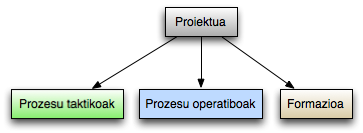
\includegraphics[scale=0.6]{Pictures/Chapter3/LDE.png}
\caption{Lanaren deskonposaketa egitura diagrama}
\label{lde}
\end{center}
\end{figure}
\begin{figure}[htp]
\begin{center}
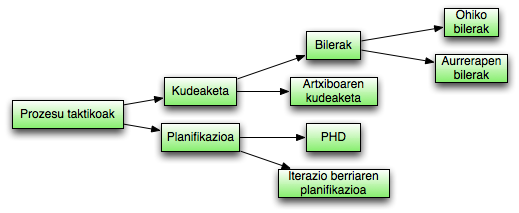
\includegraphics[scale=0.5]{Pictures/Chapter3/LDE-PT.png}
\caption{LDE - Prozesu taktikoak}
\label{lde-pt}
\end{center}
\end{figure}
\begin{figure}[htp]
\begin{center}
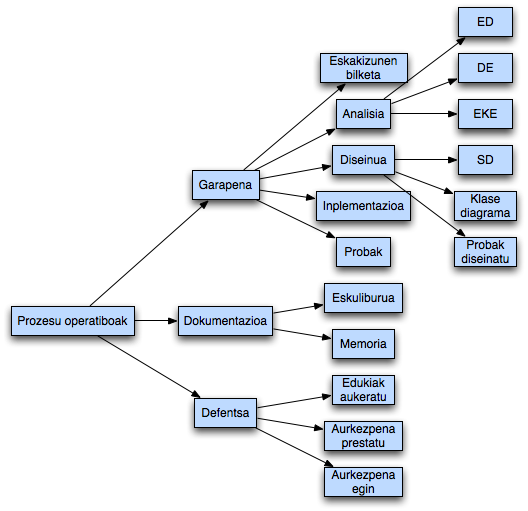
\includegraphics[scale=0.5]{Pictures/Chapter3/LDE-PO.png}
\caption{LDE - Prozesu operatiboak}
\label{lde-po}
\end{center}
\end{figure}
\begin{figure}[htp]
\begin{center}
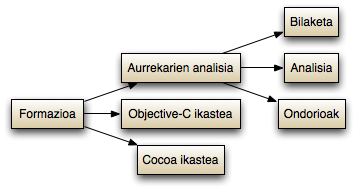
\includegraphics[scale=0.5]{Pictures/Chapter3/LDE-Formazioa.png}
\caption{LDE - Formazioa}
\label{lde-formazioa}
\end{center}
\end{figure}

\subsubsection{Azpiatazen zerrenda}
\begin{itemize}
\item \textbf{Kudeaketa:}
	\begin{itemize}
	\item K1 - Bilerak:
		\begin{itemize}
		\item K11 - Ohiko bilerak: proiektuaren jarraipenerako zuzendari eta ikaslearen artean egingo diren bilerak.
		\item K12 - Aurrerapen bilerak: iterazioa amaitzerakoan proiektuaren egoera aztertzeko bilerak.
			\begin{itemize}
			\item K121 - Bilera burutu.
			\item K122 - Egoera txostena egin.
			\end{itemize} 
		\end{itemize}
	\item K2 - Artxiboaren kudeaketa: proiektuan zehar sortutako materialaren segurtasun kopiak egitea.
	\end{itemize}
\item \textbf{Planifikazioa:}
	\begin{itemize}
	\item P1 - Proiektuaren helburu dokumentua egin.
	\item P2 - Iterazio berriaren planifikazioa: iterazio berria hasterakoan hau planifikatu behar da.
	\end{itemize}
\item \textbf{Garapena:}
	\begin{itemize}
	\item G1 - Eskakizunen bilketa: programaren eskakizun funtzionalak aztertzea.
	\item G2 - Analisia:
		\begin{itemize}
		\item G21 - Egoera diagrama egin.
		\item G22 - Erabilpen kasuen eredua egin: 
		\item G23 - Domeinuaren eredua egin.
		\end{itemize}
	\item G3 - Diseinua:
		\begin{itemize}
		\item G31 - Sekuentzia diagramak egin.
		\item G32 - Klase diagrama egin.
		\item G33 - Probak diseinatu.
		\end{itemize}
	\item G4 - Inplementazioa.
	\item G5 - Probak egin.
	\end{itemize}
\item \textbf{Dokumentazioa:}
	\begin{itemize}
	\item D1 - Memoria egin.
	\end{itemize}
\item \textbf{Defentsa:}
	\begin{itemize}
	\item B1 - Edukiak aukeratu.
	\item B2 - Aurkezpena prestatu.
	\item B3 - Aurkezpena egin.
	\end{itemize}
\item \textbf{Formazioa:}
	\begin{itemize}
	\item F1 - Aurrekarien analisia:
		\begin{itemize}
		\item F12 - Azpititulu editoreen bilaketa.
		\item F13 - Aukeratutako editoreen analisia.
		\item F14 - Konparaketa eta ondorioak.
		\end{itemize}
	\item F2 - Objective-C ikastea.
	\item F3 - Cocoa ikastea.
	\end{itemize}
\end{itemize}

\subsection{Emangarrien zerrenda}
\begin{longtable}{|p{70px}|p{250px}|p{30px}|}
\hline
\grey \textbf{Emangarria} & \grey \textbf{Deskribapena} & \grey \textbf{Ataza}\\
\hline
\endhead
\hline
\caption{\label{emangarriak}Sortuko diren emangarriak}
\endfoot
\textit{Akta} & Bilera bakoitzean tratazen diren gaien laburpena & K11\\
\hline
\textit{Egoera txostena} & Proiektuaren faseen egoera aztertzen duen dokumentua & K122\\
\hline
\textit{PHD} & Proiektua planifikatzeko hasierako unean sortutako dokumentu aldaezina & P1\\
\hline
\textit{LDE diagrama} & Ataza eta azpiataza garrantzitsuenak adierazten dituen diagrama & P1\\
\hline
\textit{Gantt diagrama} & Planifikatutako ekintzen egutegiaren adierazpide grafikoa, non ekintza bakoitzaren iraupena adierazten den & P1\\
\hline
\textit{Egoera diagrama} & Programaren egoera desberdinak adierazten dituen diagrama & G21\\
\hline
\textit{Erabilpen kasuen eredua} & Programaren portaera adierazten duen diagrama & G22\\
\hline
\textit{Domeinuaren eredua} & Domeinuan agertzen diren objektuen atributuak eta erlazioak adierazten dituen diagrama & G23\\
\hline
\textit{Sekuentzia diagramak} & Eragiketa bakoitzaren portaera adierazten duten diagramak & G31\\
\hline
\textit{Klase diagrama} & Sistemaren egitura deskribatzen duen diagrama estatikoa, non sistemako klaseak eta hauen atributu eta erlazioak agertzen diren & G32\\
\hline
\textit{Programa} & Inplementazioa amaitzean sortuko den exekutagarria & G4\\
\hline
\textit{Memoria} & Proiektuko lan guztia laburbiltzen duen dokumentua & D1\\
\hline
\textit{Aurkezpena} & Defentsan erabiliko diren gardenkiak & B2\\
\end{longtable}

\newpage
\section{Planifikazioa}

\subsection{Denboraren estimazioa}
\begin{longtable}{|l|l|}
\hline
\grey \textbf{Ataza} & \grey \textbf{Estimazioa} \textit{(orduak)}\\
\hline
\endhead
\hline
\caption{\label{estimazioa}Denboraren estimazioa}
\endfoot
\bblue Kudeaketa & \bblue 30 \\
\hline
\blue \hspace{1em}Bilerak & \blue 25 \\
\hline
\hspace{2em}Ohiko bilerak & 20 \\
\hline
\hspace{2em}Aurrerapen bilerak & 5 \\
\hline
\blue \hspace{1em}Artxiboaren kudeaketa & \blue 5 \\
\hline
\bblue Planifikazioa & \bblue 10 \\
\hline
\blue \hspace{1em}PHD egin & \blue 7 \\
\hline
\blue \hspace{1em}Iterazio berriaren planifikazioa & \blue 3 \\
\hline
\bblue Garapena & \bblue 130 \\
\hline
\blue \hspace{1em}Eskakizunen bilketa & \blue 10 \\
\hline
\blue \hspace{1em}Analisia & \blue 15 \\
\hline
\blue \hspace{1em}Diseinua & \blue 40 \\
\hline
\blue \hspace{1em}Inplementazioa & \blue 40 \\
\hline
\blue \hspace{1em}Probak egin & \blue 25 \\
\hline
\bblue Dokumentazioa & \bblue 60 \\
\hline
\blue \hspace{1em}Memoria egin & \blue 60 \\
\hline
\bblue Defentsa & \bblue 10 \\
\hline
\bblue Formazioa & \bblue 60 \\
\hline
\blue \hspace{1em}Aurrekarien analisia & \blue 10 \\
\hline
\blue \hspace{1em}Objective-C ikasi & \blue 30 \\
\hline
\blue \hspace{1em}Cocoa ikasi & \blue 20 \\
\hline
\grey \textbf{Guztira} & \grey 300 ordu \\
\end{longtable}

\subsection{Denbora plangintza: GANTT diagrama}
Hurrengo orrialdeko \ref{gantt.osoa}~Irudian agertzen da proiektuaren denbora plangintza.

Ikusten denez, proiektuaren garapena 2009. urteko udarako dago planifikatuta, kurtsoa amaitzerakoan. Dena den, kurtsoan zehar formazioa eta beste zenbait gauza egingo dira udan garapenarekin zuzenean hasi ahal izateko.

Aurreko grafikoan oso ondo ikusten ez denez, \ref{gantt.txikia}~Irudian agertzen da udan egingo denaren denbora plangintza.

\begin{figure}[htp]
\begin{center}
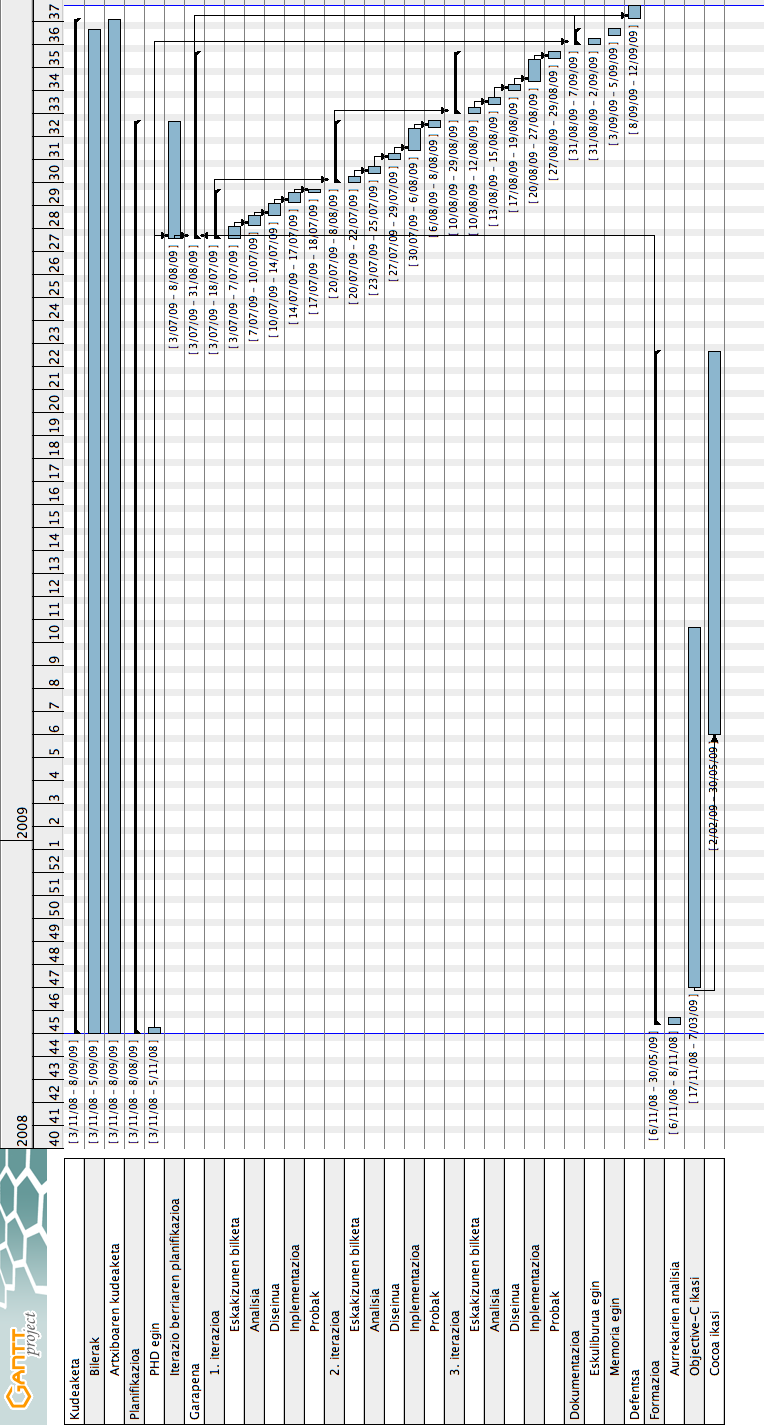
\includegraphics[scale=0.4]{Pictures/Chapter3/Gantt-osoa.png}
\caption{Gantt diagrama - Osoa}
\label{gantt.osoa}
\end{center}
\end{figure}

\begin{figure}[htp]
\begin{center}
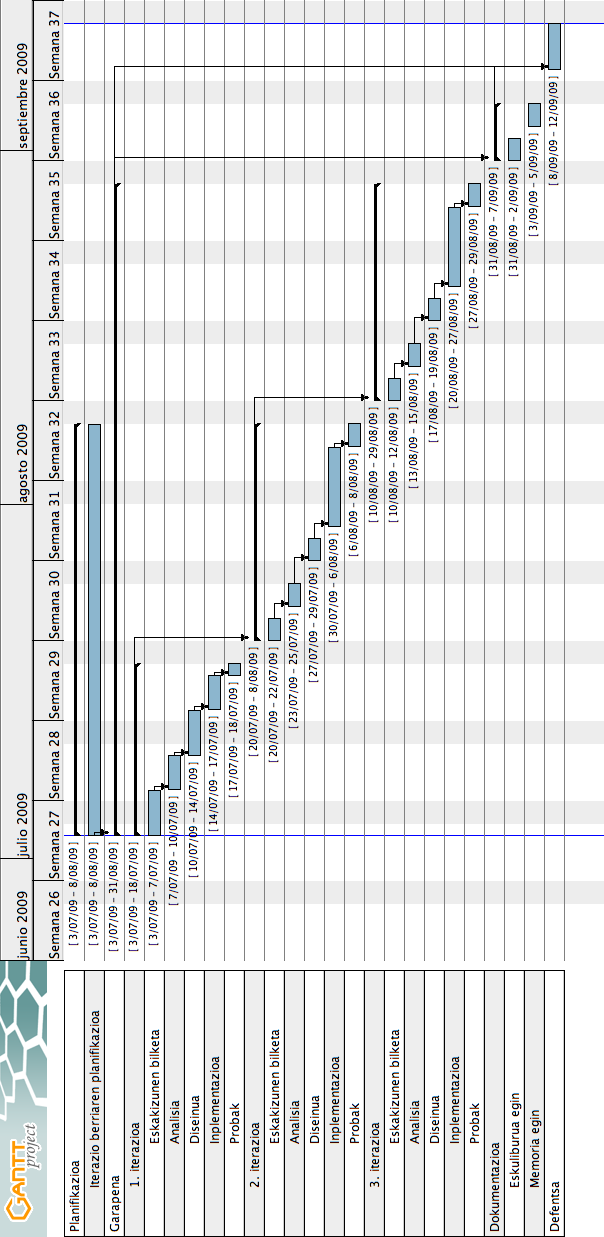
\includegraphics[scale=0.46]{Pictures/Chapter3/Gantt-txikia.png}
\caption{Gantt diagrama - Uda}
\label{gantt.txikia}
\end{center}
\end{figure}

\section{Arriskuak}
Proiektu guztietan kontuan hartu beharreko arriskuan agertzen dira, batzuk beste batzuk baino larriagoak eta gertatzeko probabilitate handiago edo txikiagokoak. Hauek dira aurreikusten diren arriskuak eta gertatzekotan zer egin behar den:
\begin{enumerate}

\item \textit{Ikasle edo irakaslearen baja gaixotasunagatik:}\\
Ikaslea gaixotzen bada, ezin izango du proiektuan lan egin. Irakaslea aldiz gaixotzen bada, ezin izango du ikaslea gidatu proiektuan zehar.\\
\textbf{Probabilitatea:} baxua.\\
\textbf{Ondorioak:} planifikatutako emangarrien atzerapenak.\\
\textbf{Konponbidea:} esfortzua birplanifikatu entregatze datak betetzeko.

\item \textit{Lan egiteko zerbitzaria atzigarri ez egotea:}\\
Assembla.com erabiliko da garapenean zehar honen tresnak erabiliz, adibidez SVN zerbitzaria han egongo da. Software edo hardware arazoak direla eta agian ezin izango da atzitu denbora tarte batean.\\
\textbf{Probabilitatea:} baxua.\\
\textbf{Ondorioak:} egindako lanaren galera eta lana ezin egitea.\\
\textbf{Konponbidea:} aurretik sortutako babes kopiak erabiltzea.

\item \textit{Garatu beharrekoaren eskakizunak aldatzea:}\\
Horrelako programetan ikasleak esperentzia nahikoa ez duenez, eskakizunen bilketa okerra egitea gerta daiteke.\\
\textbf{Probabilitatea:} ertaina.\\
\textbf{Ondorioak:} proiektuaren garapenean atzerapenak.\\
\textbf{Konponbidea:} proiektuaren helburuak birdefinitu behako lirateke edo finkatutako epeak aldatu beharko lirateke.

\item \textit{Garapenerako behar diren makinak haustea:}\\
Proiektuaren atal gehienak edozein sistema eragiletan egin daiteke, baina inplementazioa Mac OS X sisteman egitea aukeratu denez, makina espezifikoak behar dira.\\
\textbf{Probabilitatea:} oso baxua.\\
\textbf{Ondorioak:} zenbait ataza ezin izango dira aurrera eraman eta atzerapenak egongo dira.\\
\textbf{Konponbidea:} Bi makina funtzional dauzka ikasleak proiektua garatu ahal izateko. Baten bat apurtzerakoan konpontzen dagoen bitartean beste makinarekin lan egiten jarraitu daiteke.
\end{enumerate}

\section{Lan metodologia}
Proiektu honetan zehar jarraituko den metodologia softwarearen garapenerako prozesu bateratuak (\textbf{SGPB}) definitzen duena izango da. Modelatzeko lengoaia bezala \textit{Unified Modeling Language} (UML) erabiliko da.
\subsection{Bilerak}
Bilerak astean behin edo bi astero egingo dira, lan zamaren menpe. Bilera hauetan ikaslea eta proiektuaren zuzendaria egongo dira. Bertan, aste horretan egindakoa berrikusiko da planifikatutakoarekin bat datorren ikusteko eta hurrengo bileraren data esleituko da. Honez gain, denbora tarte horretan zein ataza egingo diren planifikatutko da.
\subsection{Teknologiak / Softwarea}
Proiektu honen garapenerako teknologia eta software hauek erabiliko ditugu:
\begin{itemize}
\item \textbf{\LaTeX{}:} dokumentazioa sortzeko markaketa lengoaia. WYSIWYM\footnote{\textit{What You See Is What You Mean} - Ikusten duzuna da egin nahi duzuna. \url{http://en.wikipedia.org/wiki/WYSIWYM}} motakoa da eta dokumentazioa teknikoa sortzeko oso erabilia da. Lana erraztearren, \textbf{itsas}\footnote{\url{http://itsas.ehu.es/}} taldeak eskaintzen duen txantiloia erabiliko da, bertan memoriak eduki behar duen formatua oso ondo definituta dagoelako eta lan asko aurreratuko digulako.

\LaTeX{} lengoaia da soilik, beraz editore bat eta konpiladore bat (iturburu fitxategietatik PDF fitxategi bat lortzeko) beharko ditugu. Editore bezala \textbf{MacVim}\footnote{\url{http://code.google.com/p/macvim}} erabiliko da, Mac OS X-erako vim editore famatuaren bertsio bat. Konpilatzeko \textbf{Mac\TeX}\footnote{\url{http://www.tug.org/mactex/}} distribuzioa erabiliko da, bertan beharko ditugun tresna eta plugin guztiak aurkituko ditugulako.
\item \textbf{iWork:} ofimatikarako suite bat. Nahiz eta \LaTeX{} erabili dokumentazioa sortzeko, behar bada erabili behar izango dugu, adibidez grafikoak sortzeko.
\item \textbf{Dia:} diagramak sortzeko tresna. Gure kasuan UML erabiliko dugunez zenbait diagrama sortu beharko ditugu proiektuan zehar: LDE, EKE, sekuentzia diagramak, klase diagramak, etab.
\item \textbf{GanttProject:} Gantt diagrama sortzeko erabiliko dugu, hau da, proiektuaren ataza desberdinen iraupena deskribatzeko.
\item \textbf{Objective-C 2.0:} objektuei zuzendutako programazio lengoaia, C lengoaiaren gainean eratua. Mac OS X sisteman aplikazioak garatzeko programazio lengoaia erabiliena da. Konpilatzeko ez dugu ezer berezirik behar, \textbf{gcc} konpiladore famatua erabili daitekeelako.

2.0 bertsioan asko lagunduko diguten funtzionalitateak aurkituko ditugu: zabor bilketa, propietateak, \textit{fast enumeration}, etab.

Lengoaia ikasteko liburu bat erabili da, bibliografian aipatzen dena \cite{ko:08}.
\item \textbf{Cocoa:} objektuei zuzendutako API\footnote{Application Programming Interface} natiboa Mac OS X sistemarako. Objective-C lengoaia erabiltzen du eta sistemarekin bikain integratzen dira API hau erabiltzen duten aplikazioak.

Cocoa ikasteko liburu bat erabili da, bibliografian aipatzen dena \cite{hi:08}.
\item \textbf{Xcode:} aplikazioa garatzeko IDE\footnote{Integrated Development Environment}-a. Beste IDE gehienetan aurkitu ditzakegun funtzionalitateak dauzka (araztailea, sintaxi koloreztailea, etab.).
\item \textbf{Interface Builder:} Cocoa aplikazioen interfaze grafikoak eratzeko eta kodearekin \textit{lotzeko} aplikazioa. Bi aplikazio hauek eta gcc konpiladorea Apple-ek eskaintzen ditu dohain: \url{http://developer.apple.com/Tools/}.
\end{itemize} 
\section{Bideragarritasuna}
Ekonomikoki proiektua bideragarria da, ez dugulako dirurik inbertitu behar, garapenerako ekipoak baditugulako. Sistema eragilea kenduta, erabiliko diren tresna eta teknologia guztiak dohainekoak dira, eta horietako batzuk gainera askeak dira.

% TODO: feo feo
Ikuspegi teknologikoa kontuan hartuta ere bideragarria da, egin nahi duguna inplementatuta dagoelako beste sistema eragile batzuetan.

Azkenik, denboraren ikuspuntutik, kurtsoan zehar egitea ezinezkoa izango da, ikasleak duen lan zamagatik, beraz, proiektuaren zati handiena udan egin behar izango da, ekaineko azterketak bukatu ondoren. Plangintzaren arabera iraileko bigarren asterako prest egon beharko da.
